% 20 Apr 2014 : GWA : 1 page.

\section{Related Work}
\label{sec-related}

\begin{figure*}[t]
  \centering
  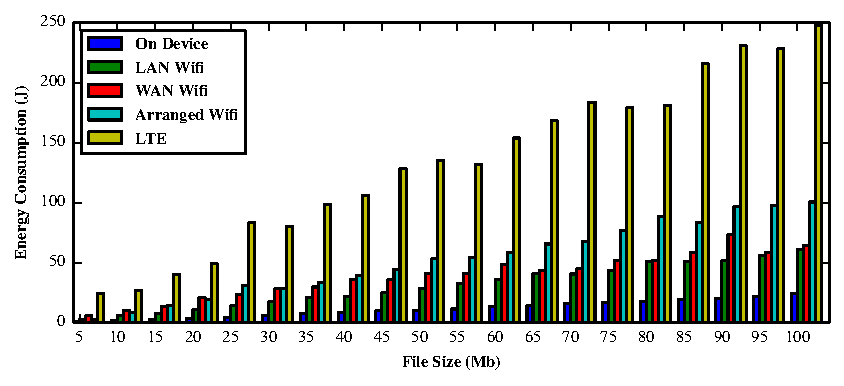
\includegraphics[width=0.8\textwidth]{./figures/energyconsumption.pdf}
  
  \vspace*{-0.1in}

  \caption{\small \textbf{PocketLocker energy consumption.}Figure illustrates the energy
  consumption on interactive device to access files of different sizes from
fixed devices in various types of network.}

  \label{fig-evaluation-energy}
  
  \vspace*{0.05in}

  \hrule

  \vspace*{-0.2in}

\end{figure*}
Mobile devices, being relatively new, did not contribute to the design of
prototype distributed file systems.  Early systems such as
Coda~\cite{kistler1992disconnected} and Ficus~\cite{guy1990implementation} were
concerned with addressing the base problem of file caching and replication.
The limitations of mobile devices, particularly constrained storage and energy
and intermittent connectivity, were not relevant.  Standard network file
systems such as NFS~\cite{nowicki1989nfs} did not provide direct offline access
or redundancy.

By contrast, there are robust commercial solutions such as
TimeMachine~\cite{timemachine} that furnish redundant storage from any device.
These cloud solutions are also typically limited in space and use third party
storage.

The approach taken by EnsemBlue~\cite{peek2006ensemblue} focuses on replicating
files among mobile devices.  Users can specify file groups that are
automatically replicated.  Cimbiosys~\cite{ramasubramanian2009cimbiosys}
narrows this approach, implementing data filters such as file type to determine
replication policy.  Files that do not match the filter are not replicated.
These approaches limit access to files that can fit on a particular user's
device.  Additionally, since a file will not always be replicated, there is no
specific attempt to provide file backup.  Since offline edits are allowed,
conflicts occur and must be resolved.  PRACTI~\cite{belaramani2006practi}
focuses on maximizing the tradeoffs of the general goals of consistency,
replication and independence.  This necessarily unfocuses the specific needs of
mobile storage.

PocketLocker aims to make all files in the PSC available.  Which files are
maintained locally are determined by usage patterns and network conditions.
Those that are not are still available with a possible delay.  The size of the
PSC can thus greatly exceed the local storage of a particular device.  The
chunk distribution system of PocketLocker minimizes the impact of device
failure and ensures file redundancy.

The Eyo system~\cite{strauss2010device} provides a distributed unified
namespace.  While file metadata is automatically replicated, replication of
file data is left to rules specified by client programs.  Thus, files may not
be replicated against failure.  If a user wants to access a nonlocal file, the
system can furnish its current location but does not automatically retrieve it.
Editing a file offline can result in a conflict that must be resolved.  The
system addresses storage pressure by pruning file version history without
respect to possible loss of redundancy.

The concept of separating the distribution of file metadata from data underpins
another system, Ori~\cite{mashtizadeh2013replication}.  Accessing remote file
data depends on being able to access that device directly.  Otherwise, the call
fails.  Ori permits users to move versioned file histories among
devices---permitting offline editing but incurring storage overhead and
producing conflicts.  File backup focuses on versioning.  Whether a file is
replicated depends upon whether the user has mounted a remote system.
Implementation of deliberate redundancy, in the form of multiple copies on
multiple devices, remains a function of user choices.  

PocketLocker handles replication of both file metadata and data directly.  The
system, having a bird's eye view of all storage devices, can ensure that files
are always chunked and replicated to disparate devices to guard against
failure.  Distribution of the chunks is tuned to the differing storage
capacities of different devices.  Storage reclamation policy follows file
history and usage patterns in order to maximize backup potential.  The
centralized design of PocketLocker also allows it to handle potential remote
access issues.  If a file or chunks are not directly reachable from a client
device due to firewall issues, the Orchestrator can often mediate an indirect
relay transfer rather than simply failing.


